
\section{Description of the model}
\label{sec:model}

In the following subsection the mathematical implant is shown, followed by a discussion of the obtained results compared to literature. Finally, the effects of the parameters are understood and presented.

\subsection{Mathematical background}
\label{ssec:math}
The notation and the model description has been already presented in \cite{MingLiu}, here a brief overview, necessary to understand the document, is given. The model framework is SEIQRS: the population of $N$ individuals are separated into these five classes. Quantities with capital letters (such as $S$, $E$\dots) indicate the real number of individuals belonging to the given class, whether quantities given wih small letters (such as $s$, $e$\dots) correspond to fractions (i.e. $s = S/N$). \\

The suscpetible $S$ class correspond to all people who can be potentially infected. In time, they decrease by the number of people getting exposed (thus in touch with an infected individual), and increased by the number of recovered people not developing immunity after being infected. The time variation of $\dot{s} = \frac{ds}{dt}$ is then:
\begin{equation}
\dot{s} (t)= -\beta\braket{k}s(t)i(t)+\gamma{r(t)} 
\end{equation} 
The exposed $E$ people are individuals got in touch with an infected. An exposed person, after $\tau$ days, they turn to infected. Then the equation for $\dot{e}$:
\begin{equation}
\dot{e} (t)= \beta\braket{k}s(t)i(t) - \beta\braket{k}s(t-\tau)i(t-\tau) 
\end{equation} 
Infected people $I$ decrease by the number of deaths and quarantined people, giving the equation for $\dot{i}$ :
\begin{equation}
\dot{i} (t)= \beta\braket{k}s(t-\tau)i(t-\tau) - d_1i(t) - \delta {i(t)}
\label{eqn:idot}
\end{equation} 
Quarantined people $Q$ may die or recover, therefore $\dot{q}$ follows the equation:
\begin{equation}
\dot{q} = \delta{i(t)} - d_2{i(t)} - \mu{i(t)}
\end{equation}
Finally, recovered people may actually turn back in susceptible, then the equation for $\dot{r}$:
\begin{equation}
\dot{r} = \mu{q(t)}-\gamma{r(t)}
\end{equation}

The small-world assumption makes all individuals interact with each other, and the numbers of interactions per day is measured by the $\braket{k}$ parameter. The initial conditions state $i(0) = i_0 \ll 1$, $e(0) = e_0 = \braket{k}i_0$ and $s(0) = s_0 = 1-i_0-e_0$. The coupled equations are solved with a second-order Runge-Kutta Method. No substantial discrepancy has been observed by using Euler method.


\subsection{Comparison with literature}
The results obtained are cross-checked with the literature \cite{MingLiu,MingLiuOld}. The input parameters are set the same as in Section~4.1 of \cite{MingLiu}, where a numerical example of the model prediction is shown. The values of the parameters are reported in Table~\ref{tab:literature_parameters}.

\begin{table}
\centering
\begin{tabular}{@{}llllll@{}}
%\cmidrule[\heavyrulewidth]{1-2} \cmidrule[\heavyrulewidth]{4-5}
\toprule
%Parameter & Value & \phantom{aaa} & Parameter & Value \\
\multicolumn{5}{l}{Values of parameters in literature}\\
%\cmidrule{1-2} \cmidrule{4-5}
\midrule
$\beta$ & $2\times10^{-5}$ & \phantom{aaa} & $\braket{k}$ & $6$ \\
$\gamma$ & $2\times10^{-4}$ & \phantom{aaa} & $\delta$ & $0.3$ \\
$d_1$ & $5\times10^{-3}$ & \phantom{aaa} & $d_2$ & $1\times10^{-3}$ \\
$\tau$ & $5$ & \phantom{aaa} & & \\ [2mm]
$N$ & $10^4$ & \phantom{aaa} & $i_0$ & $1\times10^{-3}$\\
%\cmidrule[\heavyrulewidth]{1-2} \cmidrule[\heavyrulewidth]{4-5}
\bottomrule
\end{tabular}
\caption{Set of parameters used in literature \cite{MingLiu,MingLiuOld}.}
\label{tab:literature_parameters}
\end{table}

The evolution of the population classes obtained by solving the set of coupled equation in Section~\ref{ssec:math} is shown in Figure~\ref{fig:model_literature}. A clear difference of the evolution of the populations is evident with respect to figures in \cite{MingLiu}, where the outbreak occurs with a peak after $35$ days with a maximum of around $20\%$ of population infected. In this case, the initial infected class of population dies down in around ten days. The motivation is that the initial infected population is too low with respect to the outbreak parameter ($k\braket{k}$) and the fraction of quarantined people. \\

A confirmation that the outbreak should not spread with the used parameters is extracted directly from the equation in Section~\ref{sec:model}. A necessary condition to make let the outbreak spread is to have a positive increase of the infected population, so $\dot{i}(0)>0$. This provides an equation connecting the model parameters and the initial conditions:

\begin{equation}
i_0 > \frac{\left(\delta+d_1\right)-\beta\braket{k}}{\beta\braket{k}(1+\braket{k})}
\label{eqn:i0dotgtr0}
\end{equation}

Therefore there is a threshold to the initial infected population to make the outbreak occur. From Equation~\ref{eqn:i0dotgtr0}, one see that a higher quarantine fraction and mortality ask for higher initial infected population. Also, since $\beta\braket{k}\ll1$, a smaller $\beta\braket{k}$ asks for higher initial infected population. Setting the model parameters to Table~\ref{tab:literature_parameters}, $i_0>360$, that is meaningless, since it is expected to be lower than $1$. By imposing this condition, a relation between the different parameters is also found: 
\begin{equation}
\beta > \frac{\delta + d_1}{\braket{k}(\braket{k}+2)}
\label{eqn:i0low1}
\end{equation}
This condition is necessary to provide meaningful values of the population fractions. Using $\delta$, $d_1$ and $\braket{k}$ from Table~\ref{tab:literature_parameters}, $\beta>6\times10^{-3}$ and $i_0\approx1$, that is a limit case. Probably the $\beta$ parameter is scaled up of orders of magnitudes according with the initial conditions. The $\beta$ parameter is then scaled up to a reasonable value to make the outbreak happen, setting all the other parameters to Table~\ref{tab:literature_parameters}. Since one wants $i_0\ll1$, then:

\begin{equation}
i_0<1 \Rightarrow \beta\gg \frac{\delta + d_1}{\braket{k}(\braket{k}+2)} \approx \frac{\delta}{\braket{k}(\braket{k}+2)} \approx \frac{0.3}{48} \approx 6\times10^{-3}
\label{eqn:numerical_i0low1}
\end{equation}

But also: 

\begin{equation}
\dot{i}(0)>1 \Rightarrow \beta > \frac{\delta + d_1}{\braket{k}\left[1+\left(1+\braket{k}\right)i_0\right]} \approx \frac{\delta}{\braket{k}} \approx \frac{0.3}{6} \approx 5\times10^{-2}
\label{eqn:numerical_i0dotgtr1}
\end{equation}

Assuming the difference is a matter of order of magnitude in the $\beta$ parameter, $\beta$ is set to $0.2$. The corresponding evolution is shown in Figure~\ref{fig:model_literature_modified}: a similar evolution as in \cite{MingLiu} is observed.

\begin{figure}[!ht]\centering
\subfloat[\label{fig:model_literature}
]{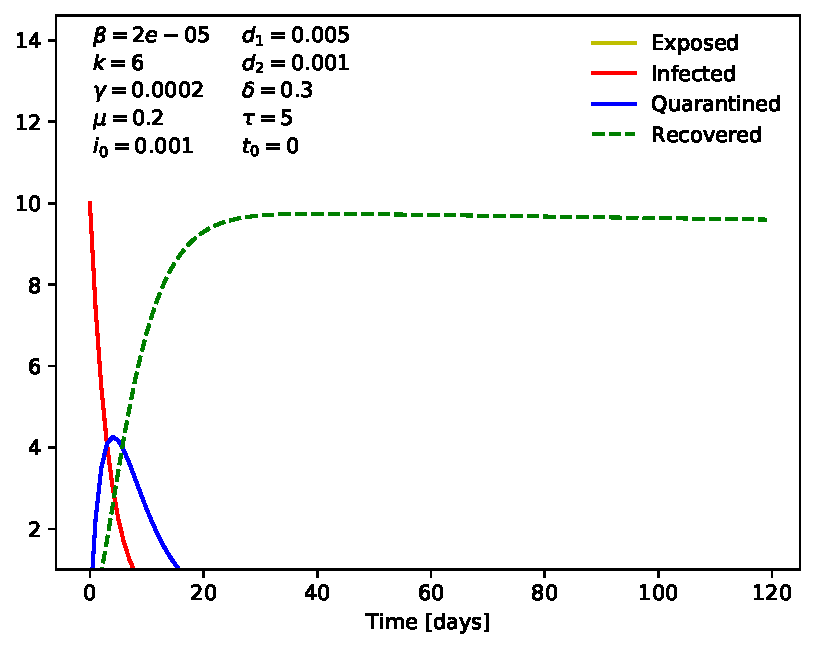
\includegraphics[width=0.4\textwidth]{imgs/ModelDescription/Summary_parameters_nominal.pdf}}
\subfloat[\label{fig:model_literature_modified}
]{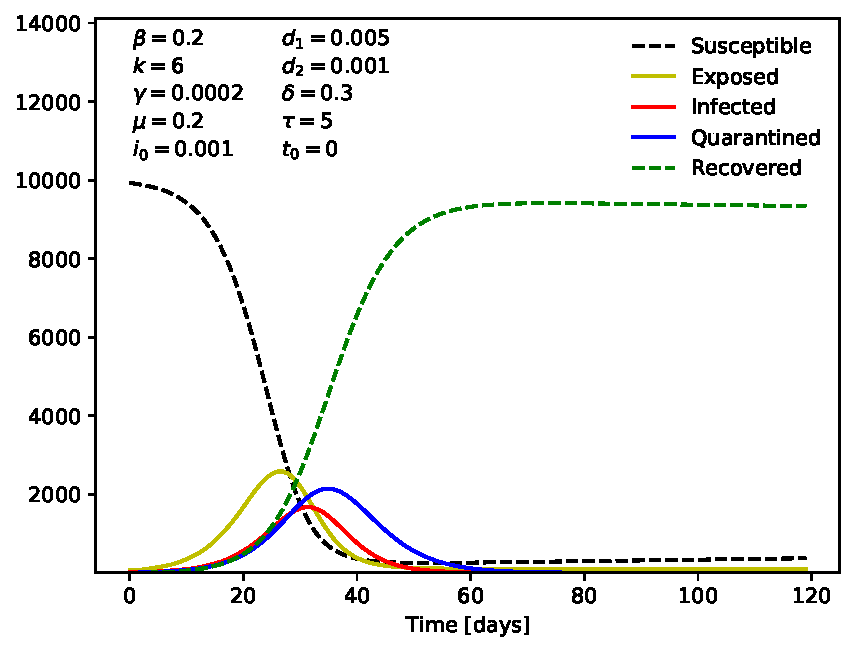
\includegraphics[width=0.42\textwidth]{imgs/ModelDescription/Summary_parameters_alternative.pdf}}
\caption{Numerical prediction of the model with different settings of the parameters. Parameters in Table~\ref{tab:literature_parameters} are used in (a), as well as in (b) but for $\beta=0.2$.}.
\end{figure}


\subsection{Impact of parameters on model predictions}
In this subsection the impact of the parameters on the model predictions is analysed. The most important parameters for the evolution of the infected population and the occurrence of the outbreak are $\beta$ and $\braket{k}$ parameters. The $\beta$ parameters is connected to the infection factor, so the probability of infecting a susceptible person in contact with and infected one. The $\braket{k}$ parameters indicate instead the number of connection for each individual, so measures the level of interaction of the small world. Since the two parameters always come together their effect is the same on the evolution and visible in Figure~\ref{fig:scan_i_vs_beta}, the larger those parameters are the steeper is the curve of the infected population, as expected from Equation~\ref{eqn:idot}.  A large impact on the outbreak evolution is also given by the fraction of quarantined infected population $\delta$, as shown in Figures~\ref{fig:scan_i_vs_delta} and \ref{fig:scan_q_vs_delta}. The outbreak is significantly contained in case a larger fraction of infected population is spotted and quarantined.

\begin{figure}[!ht]\centering
\subfloat[\label{fig:scan_i_vs_beta}]{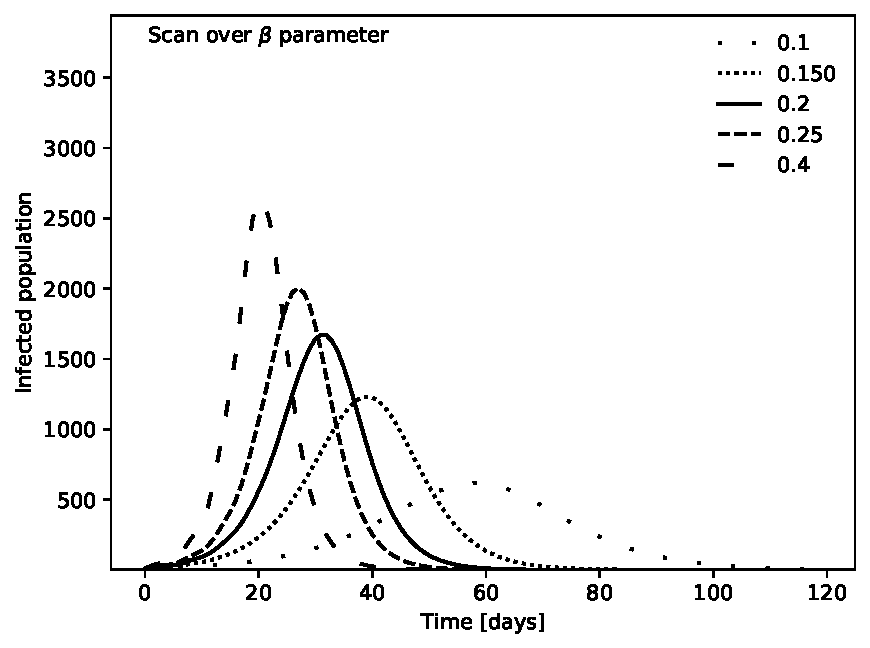
\includegraphics[width=0.32\textwidth]{imgs/ModelDescription/Scan_I_vs_beta_parameters_alternative.pdf}}
\subfloat[\label{fig:scan_i_vs_delta}]{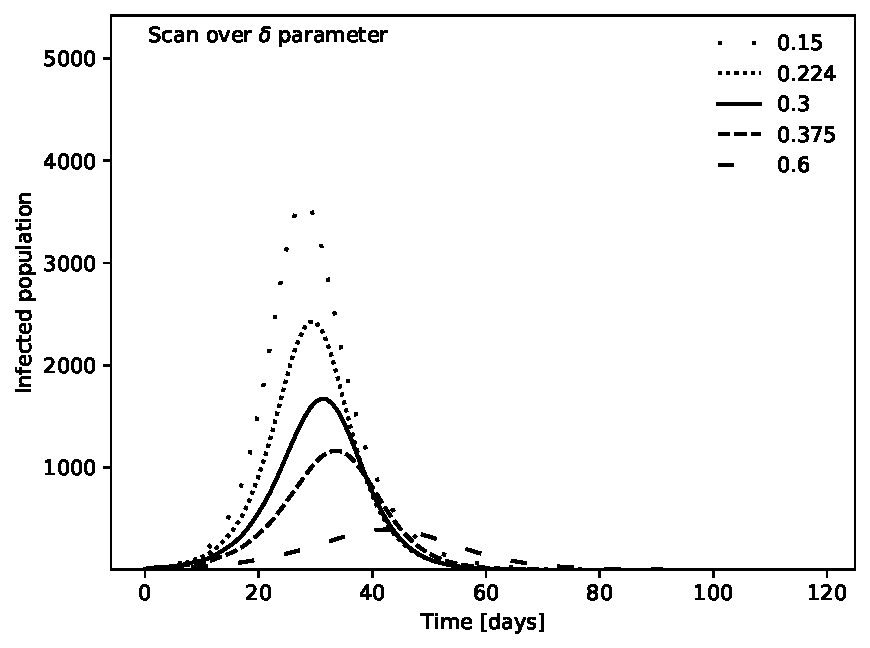
\includegraphics[width=0.32\textwidth]{imgs/ModelDescription/Scan_I_vs_delta_parameters_alternative.pdf}}
\subfloat[\label{fig:scan_q_vs_delta}]{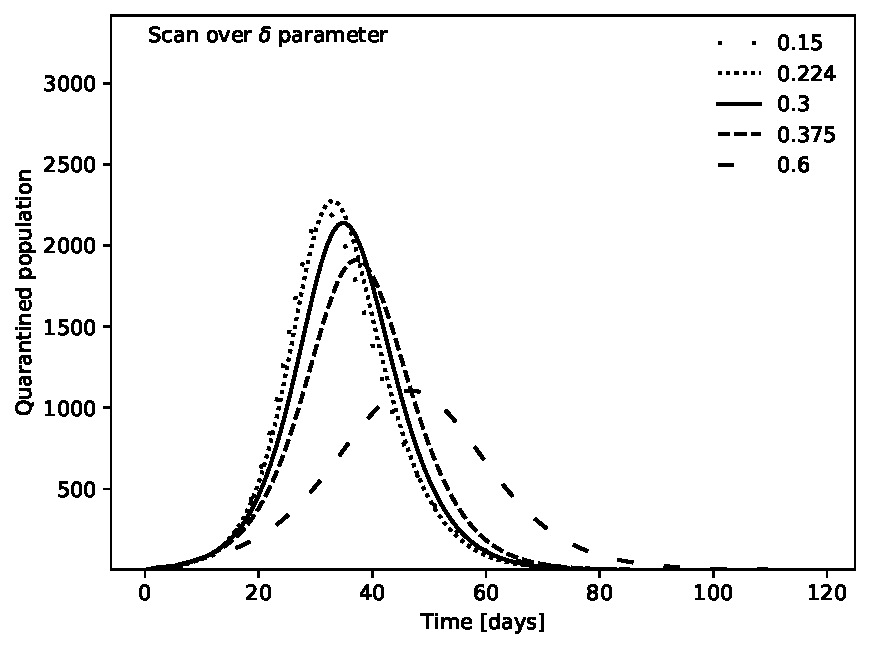
\includegraphics[width=0.32\textwidth]{imgs/ModelDescription/Scan_Q_vs_delta_parameters_alternative.pdf}}
\caption{Effect on the evolution of the infected population given by varying the $\beta$ parameter (a). Effect on infected (b) and quarantined (c) population given by varying the $\delta$ parameter.}.
\end{figure}

Other effects are given by $\gamma$, $\mu$ and $d_{1/2}$ parameters. Those control more the recovery curve. The $\gamma$ parameter is related to the probability of a recovered individual to not develop immunity: as shown in Figure~\ref{fig:scan_r_vs_gamma}, the recovered people has a decrease after the peak of the outbreak. The recovery curve is strongly affected by the $\mu$ parameter that regulates the recovery probability of the infected population: as shown in Figure~\ref{fig:scan_r_vs_mu}. The mortality $d_{1/2}$ instead increases the number of deaths, given by the difference of the recovered population and the initial $10000$ susceptible people, shown in Figure~\ref{fig:scan_r_vs_d1}.

\begin{figure}[!ht]\centering
\subfloat[\label{fig:scan_r_vs_gamma}]{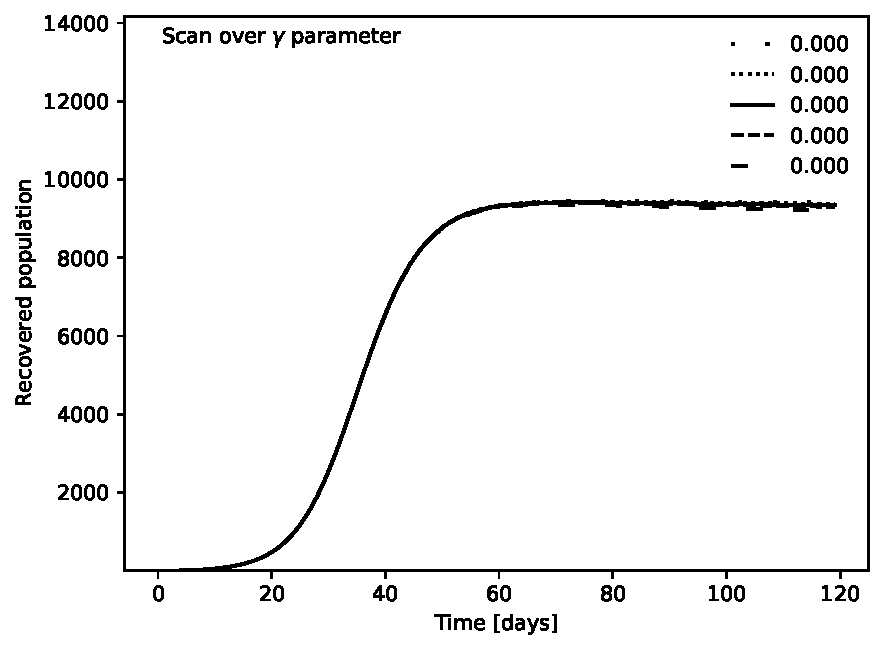
\includegraphics[width=0.32\textwidth]{imgs/ModelDescription/Scan_R_vs_gamma_parameters_alternative.pdf}}
\subfloat[\label{fig:scan_r_vs_mu}]{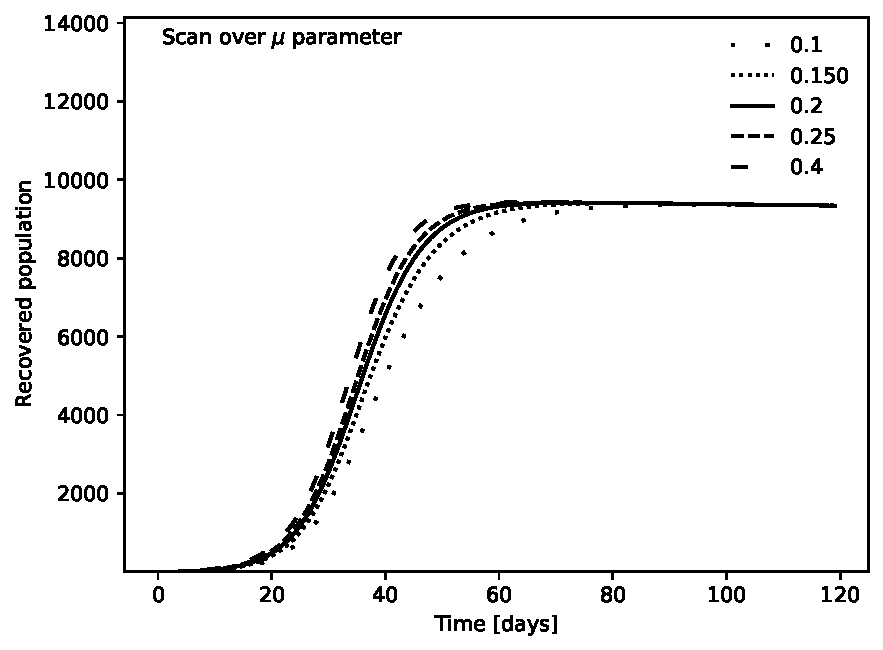
\includegraphics[width=0.32\textwidth]{imgs/ModelDescription/Scan_R_vs_mu_parameters_alternative.pdf}}
\subfloat[\label{fig:scan_r_vs_d1}]{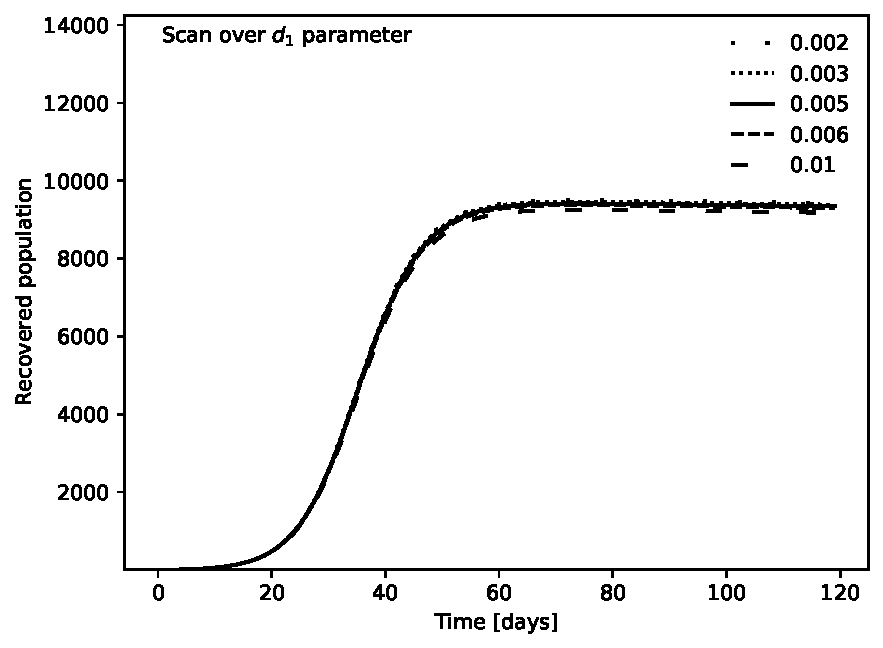
\includegraphics[width=0.32\textwidth]{imgs/ModelDescription/Scan_R_vs_d1_parameters_alternative.pdf}}
\caption{Effect on the evolution of the recovered population given by varying the $\gamma$ (a), $\mu$ (b) and $d_1$ (c) parameters.}.
\end{figure}

The only temporal parameter is the incubation time $\tau$: it also strongly affects the evolution of the oubreak, shown in Figure~\ref{fig:scan_i_vs_tau}. In case of long incubation time, the outbreak develops a  multiple peak structure, while in case of a short incubation time a clean gaussian peak is recognised.

\begin{figure}[!ht]\centering
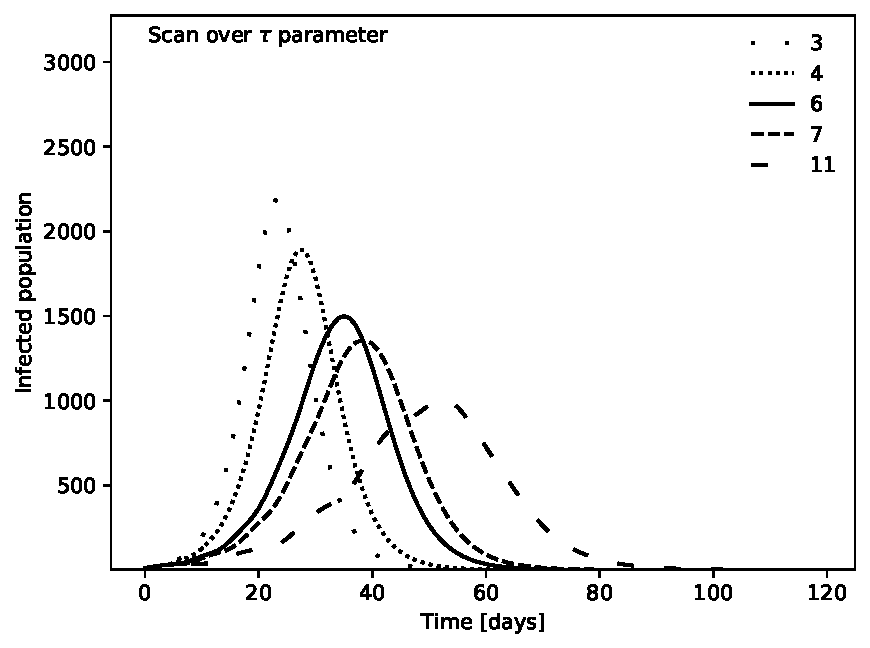
\includegraphics[width=0.4\textwidth]{imgs/ModelDescription/Scan_I_vs_tau_parameters_alternative.pdf}
\caption{Effect on the evolution of the infected population given by varying the $\tau$ parameter.}
\label{fig:scan_i_vs_tau}
\end{figure}

